\documentclass[12pt,letterpaper]{article}
\usepackage[utf8]{inputenc}
\usepackage[spanish]{babel}
\usepackage{graphicx}
\usepackage[left=2cm,right=2cm,top=2cm,bottom=2cm]{geometry}
\usepackage{graphicx} % figuras
% \usepackage{subfigure} % subfiguras
\usepackage{float} % para usar [H]
\usepackage{amsmath}
%\usepackage{txfonts}
\usepackage{stackrel} 
\usepackage{multirow}
\usepackage{enumerate} % enumerados
\renewcommand{\labelitemi}{$-$}
\renewcommand{\labelitemii}{$\cdot$}
% \author{}
% \title{Caratula}
\begin{document}

% Fancy Header and Footer
% \usepackage{fancyhdr}
% \pagestyle{fancy}
% \cfoot{}
% \rfoot{\thepage}
%

% \usepackage[hidelinks]{hyperref} % CREA HYPERVINCULOS EN INDICE

% \author{}
\title{Caratula}

\begin{titlepage}
\begin{center}
\large{UNIVERSIDAD PRIVADA DE TACNA}\\
\vspace*{-0.025in}
\begin{figure}[htb]
\begin{center}

\includegraphics[width=8cm]{./Imagenes/logo}
\end{center}
\end{figure}
\vspace*{0.15in}
INGENIERIA DE SISTEMAS  \\

\vspace*{0.5in}
\begin{large}
TITULO:\\
\end{large}

\vspace*{0.1in}
\begin{Large}
\textbf{INFORME DE LABORATORIO No 05} \\
\end{Large}

\vspace*{0.3in}
\begin{Large}
\textbf{CURSO:} \\
\end{Large}

\vspace*{0.1in}
\begin{large}
BASE DE DATOS II\\
\end{large}

\vspace*{0.3in}
\begin{Large}
\textbf{DOCENTE(ING):} \\
\end{Large}

\vspace*{0.1in}
\begin{large}
 Patrick Cuadros Quiroga\\
\end{large}

\vspace*{0.2in}
\vspace*{0.1in}
\begin{large}
Integrantes: \\
\begin{flushleft}
Adnner Esperilla Ruiz		\hfill	(2015050543) \\

\vspace*{0.5in}
\begin{center}
2019-Tacna\\
\end{center}

\end{flushleft}
\end{large}
\end{center}

\end{titlepage}


\tableofcontents % INDICE
\thispagestyle{empty} % INDICE SIN NUMERO
\newpage
\setcounter{page}{1} % REINICIAR CONTADOR DE PAGINAS DESPUES DEL INDICE

\section{INFORMACIÓN GENERAL} 

\begin{itemize}
\subsection{Objetivos:}
	\item Poder manejar correctatmente una  Base de Datos con Oracle.
	\item Poder instalar correctamente una instancia.
\subsection{Recursos Requeridos :}
	\item Tener la Virtualización activada en el BIOS de la PC.
	\item Tener Windows 10 64bit: Pro, Enterprise o Education,con minimo de  4GB de RAM.
	\item Tener  Docker Desktop(Necesario cumplir con los anteriores caracteristicas)
	\item Tener Oracle SQL Developer para Windows
	\item Tener Microsoft SQL Server 2017 o superior

\end{itemize}

\section{MARCO TEORICO} 

\begin{itemize}
\subsection{Docker:}
	\item Utilizar Docker realmente facilita la creación, implementación y ejecución de aplicaciones mediante el uso de contenedores. Y los contenedores permiten a un desarrollador empaquetar una aplicación con todas las partes que necesita, como bibliotecas y otras dependencias, y enviarla en un solo paquete. 
          \item Al hacerlo, el desarrollador puede estar seguro de que la aplicación se ejecutará en cualquier otra máquina Linux, independientemente de las configuraciones personalizadas que la máquina pueda tener que puedan diferir de la máquina utilizada para escribir y probar el código.
         \item Sirven para desplegar aplicaciones en un entorno virtual aislado, pero sin el overhead de tener un Sistema Operativo (SO) nuevo como se tiene en una Virtual Machine (VM).

\subsection{Oracle Database en Docker:}
	\item Los productos de Oracle son compatibles con Docker si el sistema operativo del host es Oracle Linux 7, pero no necesita usar un host OL7 para que esto funcione. Puedes ver cómo instalar Docker en OL7 .
	\item Usar imágenes de Oracle Container Registry o de Docker Store tiene la ventaja que los binarios de instalación vienen incluidos, lo que no es permitido por licencia en el resto de las distribuciones. 
\subsection{Referencias de cómo usar Oracle con Docker en Linux Y  en Windows:}
	\item Docker en Windows 10:
	\item Para usar la versión completa es necesario habilitar Microsoft Hyper-V, lo que implica deshabilitar la virtualización por hardware de nuestro PC. Si estamos usando VirtualBox en el mismo host, con este cambio deja de funcionar.
           \item Docker Toolbox no tiene esta restricción, aunque se mantiene como una versión antigua (Legacy), y Docker recomienda usar la versión completa.Otra diferencia de Docker Toolbox es que necesita una VM VirtualBox para ejecutar. Esta VM se crea de forma automática al usar Toolbox, de nombre default, y se usa como host para los containers que creemos.
 \subsection{Construir la imagen:}
	\item Antes de crear una imagen para docker podemos buscar en el registro de imágenes de docker que han creado otros usuarios y los han compartido por si hay alguna que ya se adapte a nuestras necesidades, si nos sirve alguna y es algo popular nos evitaremos tener que modificarla nosotros mismos según salgan nuevas versiones de los servicios que use. El registro de imágenes de docker es un servicio en el que los usuarios comparten y colaboran en la creación de las imágenes. Para los servicios más conocidos dispondremos ya de las imágenes como podrían ser: mysql, redis, postgresql, ubuntu, wordpress, nginx, mongodb.
                     \begin{figure}[H]
		\begin{center}
		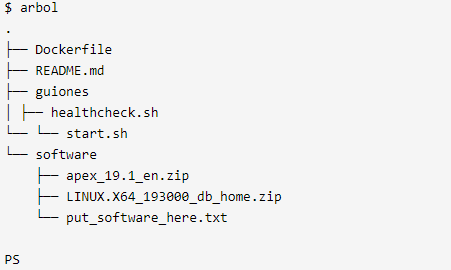
\includegraphics[width=8cm]{./Imagenes/100}
		\end{center}
		\end{figure}
	

\end{itemize}








\section{PROCEDIMIENTO} 

\begin{itemize}
\subsection{ Habriendo  Docker}
	\item Abrir el menu inicio y buscar la aplicación Docker for Windows.

	\item Ubicar la aplicación PowerShell(ejecutarla como Administrador). En la ventana de comandos de PowerShell escribir
lo siguiente.
		\begin{figure}[H]
		\begin{center}
		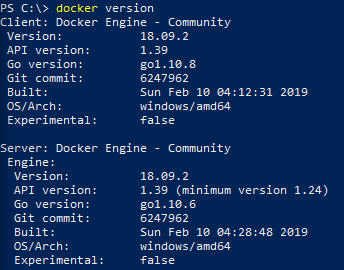
\includegraphics[width=8cm]{./Imagenes/1}
		\end{center}
		\end{figure}
     
\subsection{ Creando un contenedor con Oracle Database para Linux}
	\item Entrar a esete link (https://hub.docker.com/ )y Iniciar sesión o crear una cuenta nueva.
	\item Luego buscar  el repositorio para Oracle Database.Darle click en proceeed to  CheckOut, completar los datos y aceptar las condiciones obligatorias para obtener el acceso al contenido.
		\begin{figure}[H]
		\begin{center}
		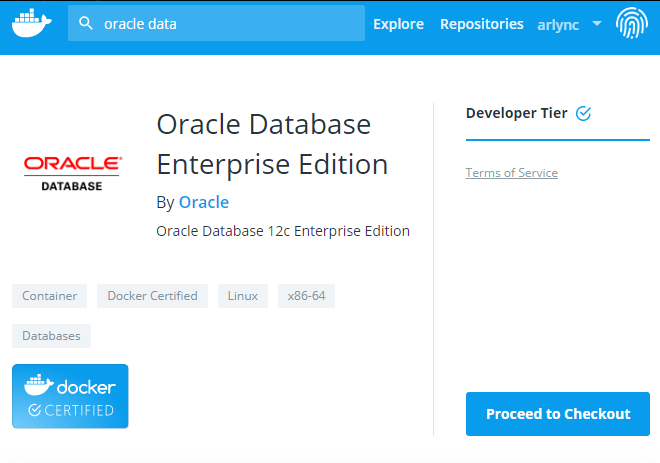
\includegraphics[width=8cm]{./Imagenes/3}
		\end{center}
		\end{figure}
	\item En la ventana de PowerShelql, escribir el siguiente comando:
		\begin{figure}[H]
		\begin{center}
		
\includegraphics[width=9cm]{./Imagenes/4}
		\end{center}
		\end{figure}
	\item Ejecutar el siguiente comando en Powershell, lo cual descargará la imagen del contenedor de Oracle Database en un servidor Linux y nos pedirra talves nuestra cuenta en docker entonces se loguea 
		\begin{figure}[H]
		\begin{center}
		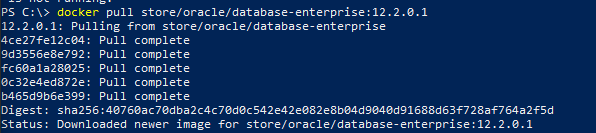
\includegraphics[width=15cm]{./Imagenes/5}
		\end{center}
		\end{figure}
	\item No aparecera como  respuesta  un ID que corresponde al contenedor.
		\begin{figure}[H]
		\begin{center}
		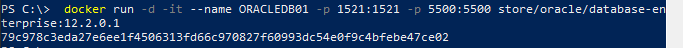
\includegraphics[width=15cm]{./Imagenes/6}
		\end{center}
		\end{figure}
	\item Verificar que el contenedor se esté ejecutando correctamente mediante el comando que ingresamos :
		\begin{figure}[H]
		\begin{center}
		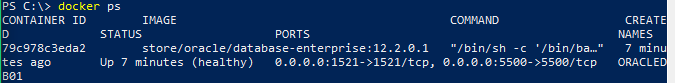
\includegraphics[width=15cm]{./Imagenes/7}
		\end{center}
		\end{figure}
	\item Cuando el estado del contenedor sea “healthy”, en la consola de Powershell, ejecutar el siguiente comando:
		\begin{figure}[H]
		\begin{center}
		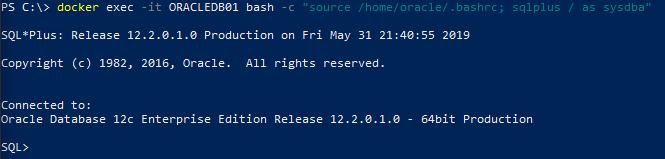
\includegraphics[width=15cm]{./Imagenes/8}
		\end{center}
		\end{figure}
	\item En la línea de comentados de SQL*Plus, escribir lo siguiente
		\begin{figure}[H]
		\begin{center}
		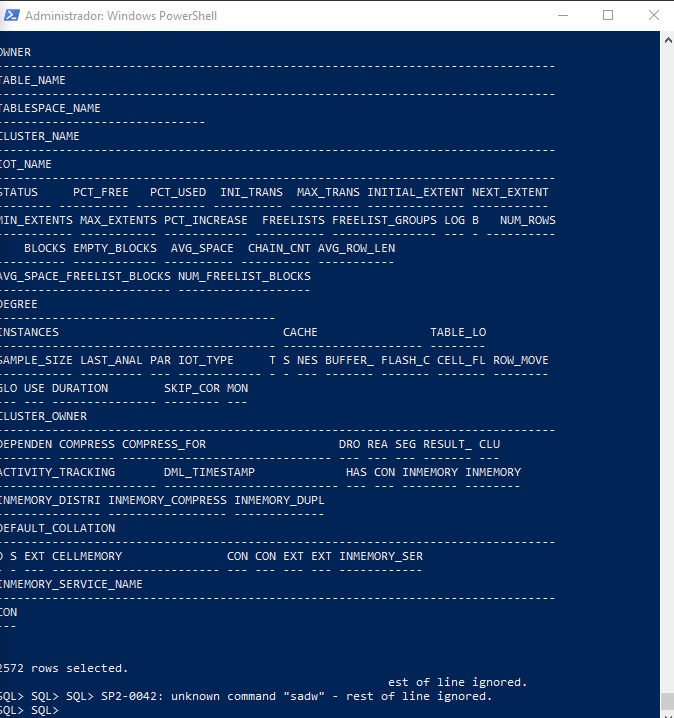
\includegraphics[width=8cm]{./Imagenes/19}
		\end{center}
		\end{figure}
	\item Escribir el comando quit para cerrar la sesión de SQL*Plus
		\begin{figure}[H]
		\begin{center}
		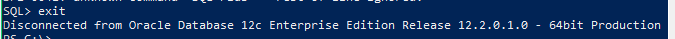
\includegraphics[width=15cm]{./Imagenes/10}
		\end{center}
		\end{figure}
	\item Ingresar a este link :https://localhost:5500/em. Iniciar sesión con los siguientes datos:
		\begin{figure}[H]
		\begin{center}
		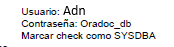
\includegraphics[width=4cm]{./Imagenes/t1}
		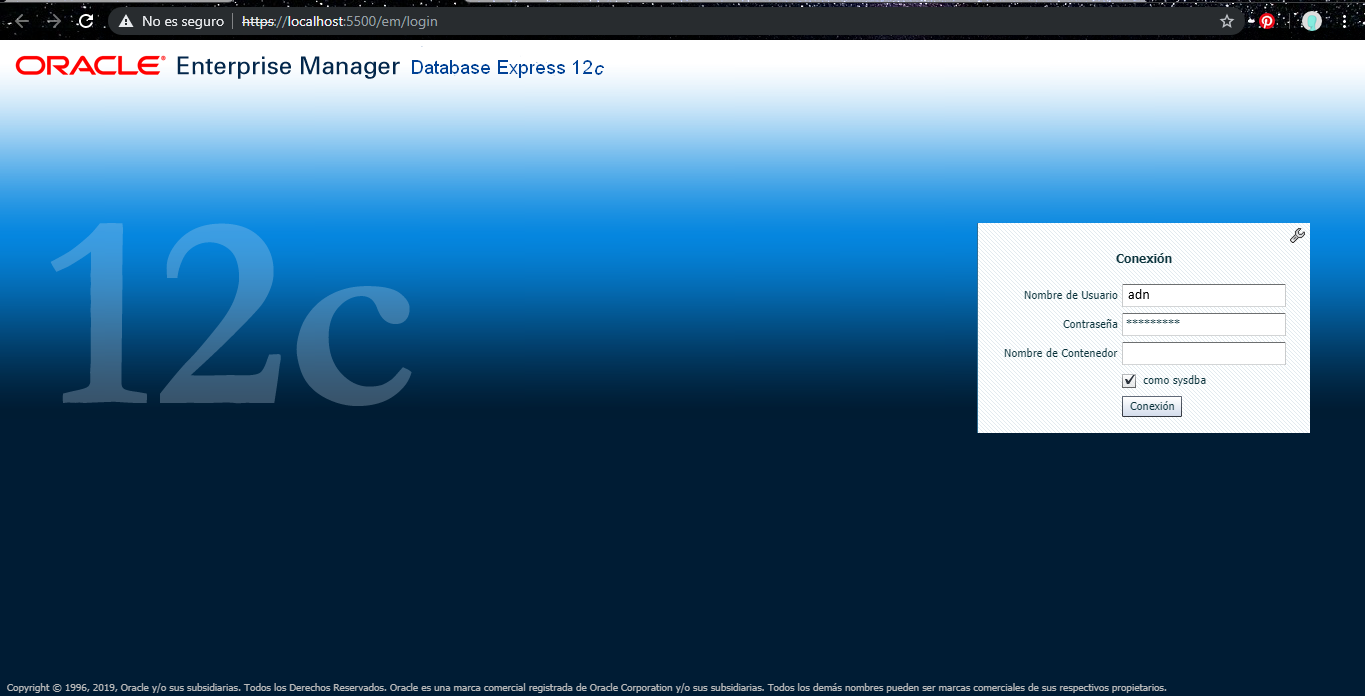
\includegraphics[width=15cm]{./Imagenes/11}
		\end{center}
		\end{figure}
	\item Luego se visualizará la siguiente ventana. Cerrar sesión y la pestaña del navegador de internet.
		\begin{figure}[H]
		\begin{center}
		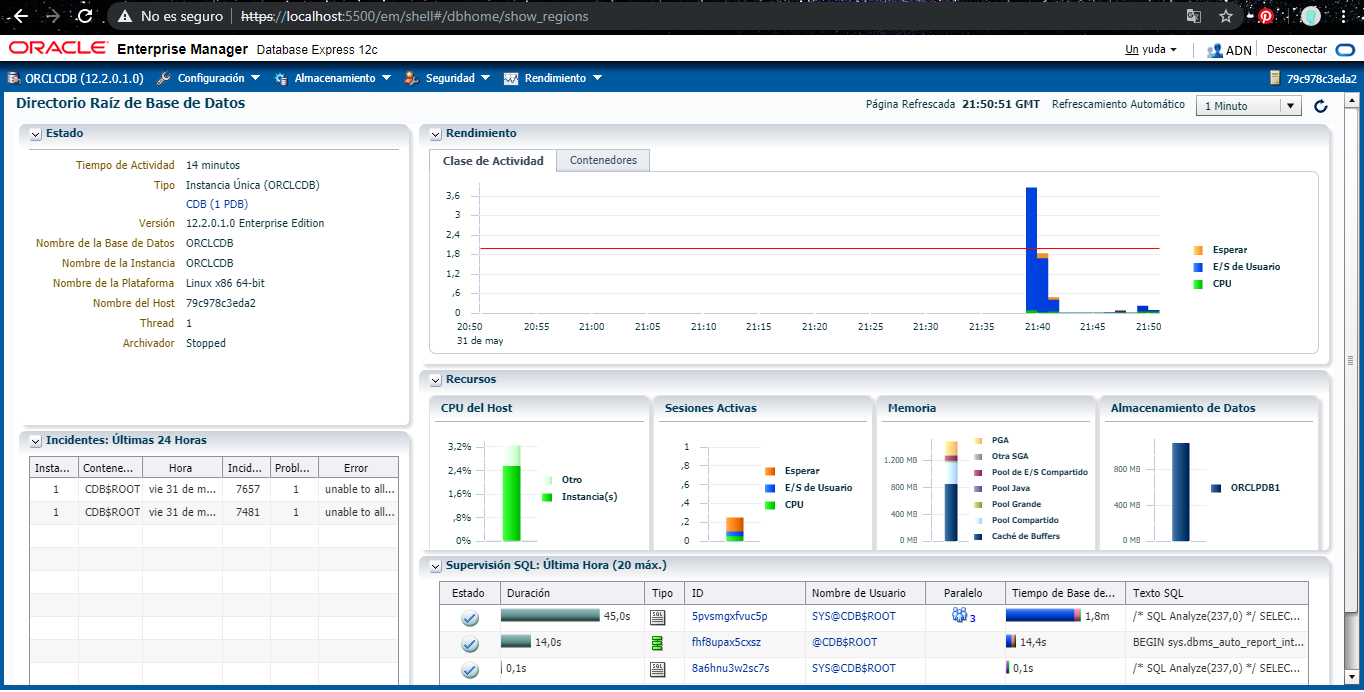
\includegraphics[width=15cm]{./Imagenes/12}
		\end{center}
		\end{figure}
	\item Iniciar el aplicativo Oracle SQL Developer y crear una nueva conexión con los siguientes parámetros:
		\begin{figure}[H]
		\begin{center}
		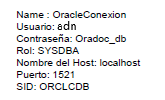
\includegraphics[width=5cm]{./Imagenes/t2}
		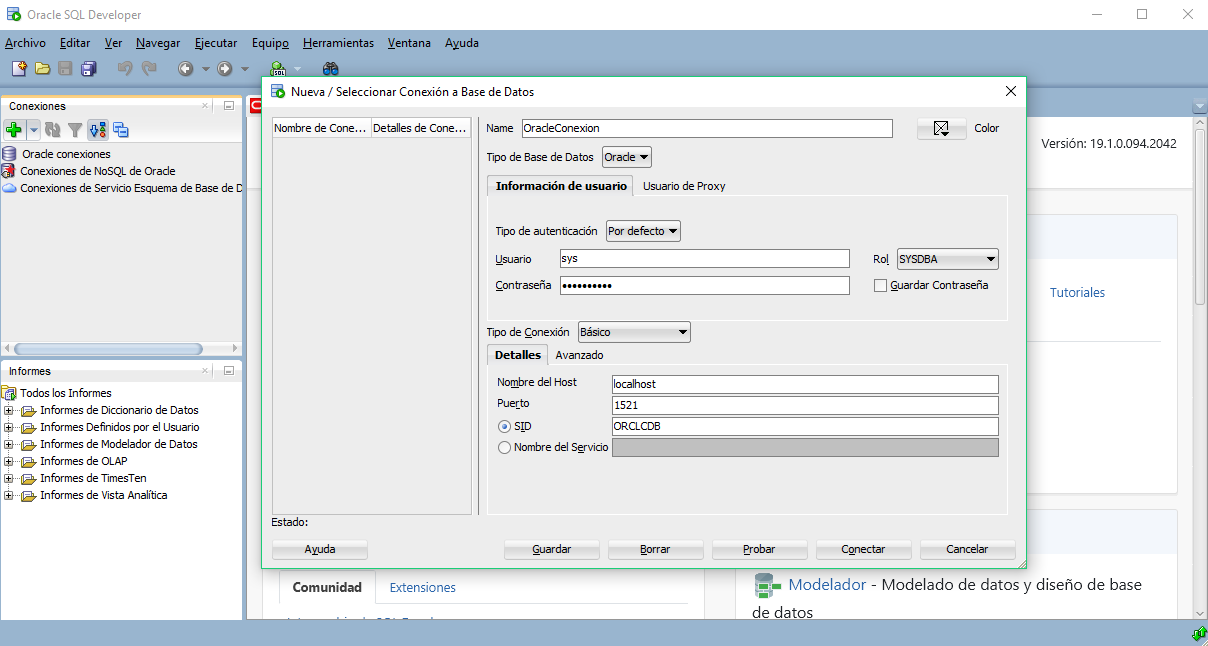
\includegraphics[width=15cm]{./Imagenes/13}
		\end{center}
		\end{figure}
	\item Damos una  nueva consulta, escribir y ejecutar lo siguiente; deberá retornar varios registros que representan las tablas de las base de datos
		\begin{figure}[H]
		\begin{center}
		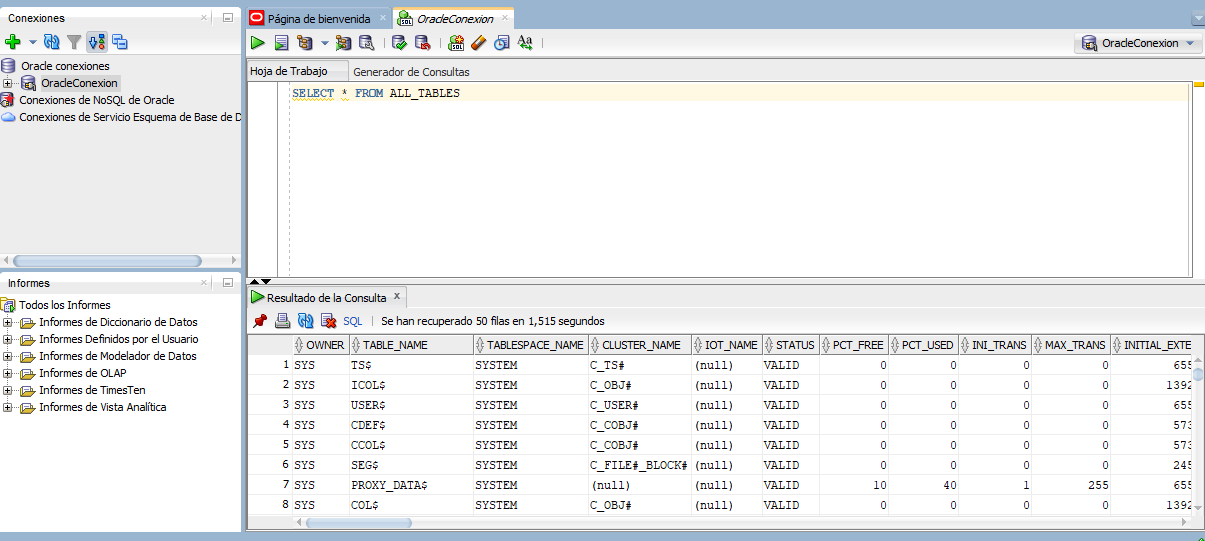
\includegraphics[width=15cm]{./Imagenes/14}
		\end{center}
		\end{figure}
	\item Cerrar la aplicación Oracle SQL Developer
	\item En PowerShell ejecutar el siguiente comando. Y verificar la eliminación del contenedor con ejecutando
		\begin{figure}[H]
		\begin{center}
		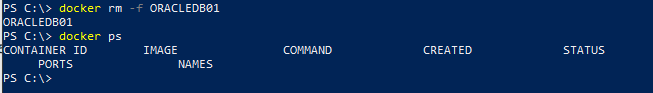
\includegraphics[width=12cm]{./Imagenes/15}
		\end{center}
		\end{figure}


\subsection{ Adicionando persistencia}
	\item En PowerShell ejecutar el siguiente comando, lo cual dara como respuesta se visualizará un ID que corresponde al contenedor
		\begin{figure}[H]
		\begin{center}
		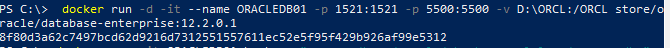
\includegraphics[width=12cm]{./Imagenes/16}
		\end{center}
		\end{figure}
	\item Repetir el paso 13 y modificar la contraseña del usuario SYS
		\begin{figure}[H]
		\begin{center}
		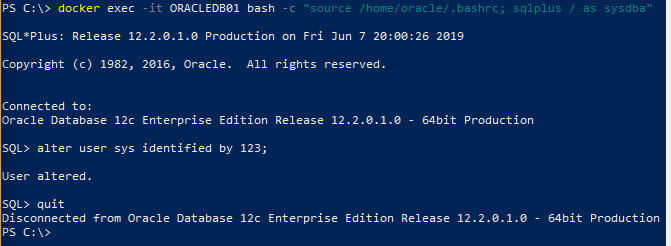
\includegraphics[width=12cm]{./Imagenes/20}
		\end{center}
		\end{figure}
       	\item Iniciar el aplicativo Oracle SQL Developer, conectarse como el usuario SYS y ejecutar el siguiente comando
		\begin{figure}[H]
		\begin{center}
		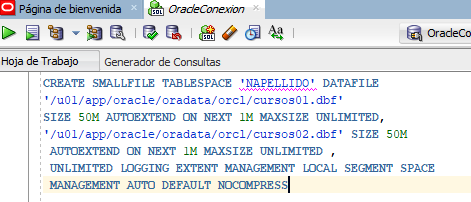
\includegraphics[width=12cm]{./Imagenes/22}
		\end{center}
		\end{figure}
	\item Verificar el contenido de la carpeta ORCL
	\item En PowerShell ejecutar el siguiente comando. Verificar la eliminación del contenedor con ejecutando
		\begin{figure}[H]
		\begin{center}
		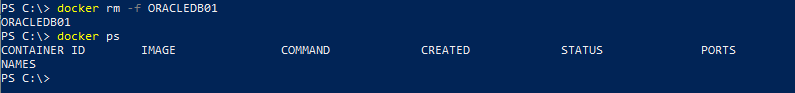
\includegraphics[width=12cm]{./Imagenes/24}
		\end{center}
		\end{figure}
	\item Cerrarmos  la aplicación Oracle SQL Developer.




\end{itemize}
		
\section{ANALISIS E INTERPRETACION DE RESULTADOS} 


\subsection{ Actividades Encargadas}
	\begin{itemize}
		\item ¿Con qué comando(s) puedo iniciar y detener una instancia de Oracle, detalle cada uno de los pasos y opciones,
utilizando Docker?
                     \item Para  Iniciar una instancia de Oracle Database Server
Iniciar una instancia de servidor de base de datos Oracle al ejecutar
" docker run -d -it --name oracle-db store/oracle/database-enterprise:12.2.0.1"donde oracle01-db está el nombre del contenedor y 12.2.0.1 es la etiqueta de imagen de Docker.
                      \begin{figure}[H]
		\begin{center}
		
\includegraphics[width=15cm]{./Imagenes/200}
		\end{center}
		\end{figure}
                      \item Los comandos docker ps -a -q detendrá todos los contenedores Docker en ejecución :
                      \begin{figure}[H]
		\begin{center}
		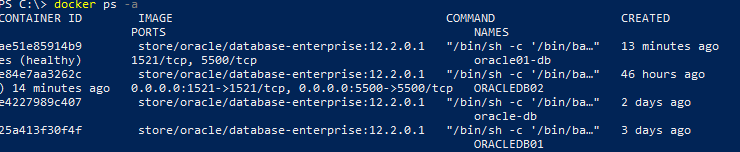
\includegraphics[width=15cm]{./Imagenes/201}
                      
\includegraphics[width=8cm]{./Imagenes/202}
		\end{center}
		\end{figure}
		\item ¿Con qué comando(s) puedo iniciar y detener el Listener y el Enterprise manager, detalle cada uno de los pasos y
opciones, utilizando Docker?
                     \item Parar iniciar el listener:" lsnrctl start"  para detener "lsnrctl stop"
                      \begin{figure}[H]
		\begin{center}
		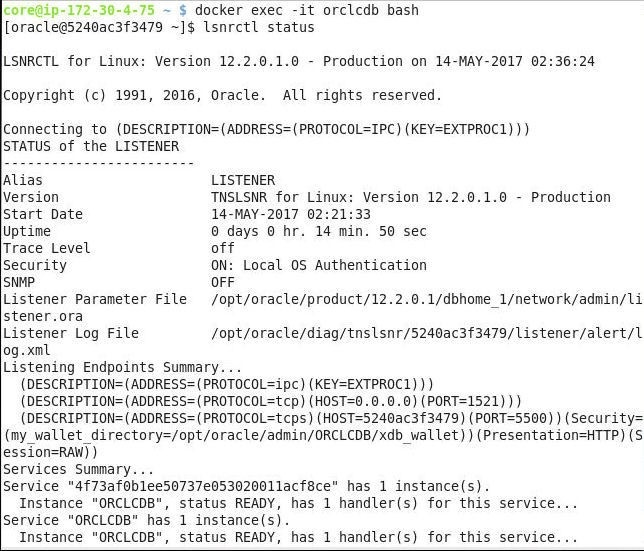
\includegraphics[width=15cm]{./Imagenes/203}
                      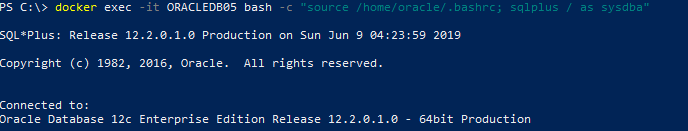
\includegraphics[width=15cm]{./Imagenes/204}
		\end{center}
		\end{figure}
		\item Genere un nuevo contenedor y cree un espacio de tablas con las siguientes características.
		\begin{figure}[H]
		\begin{center}
		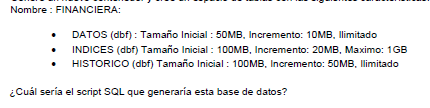
\includegraphics[width=8cm]{./Imagenes/t3}
		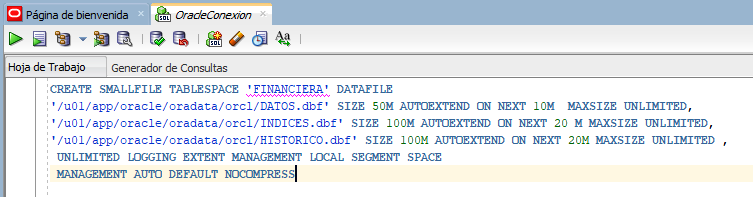
\includegraphics[width=15cm]{./Imagenes/23}
		\end{center}
		\end{figure}


	\end{itemize}




\section{CONCLUSIONES}
Como podemos ver r, hoy tenemos una tecnología disponible desde hace unos años que nos permite ir a otro nivel de virtualización distinto y mucho mas eficaz  , que nos da multiples ventajas :
\begin{itemize}
\item Instalación simple y capacidad de ejecutar múltiples aplicaciones en entornos aislados sobre un mismo sistema operativo,  permitiéndonos ahorrar horas de trabajo en la administración de Infraestructura.
\item Independiente a la plataforma, permite contar con soluciones más  rapidas y portables.
\item Despliegue de Aplicaciones mucho más rápida y flexible.
\item Disponible en múltiples proveedores de Nube .
\item Manejo de las base de datos mucho mas practicas .
	
\end{itemize}

\newpage

\section{REFERENCIAS} 

\begin{itemize}	
\item https://www.docker.com/products
         \item https://www.oracle.com/technetwork/es/articles/datawarehouse/oracle12c-docker-win10-4485487-esa.html
         \item https://picodotdev.github.io/blog-bitix/2014/11/como-crear-una-imagen-para-docker-usando-un-dockerfile/
         \item https://www.redhat.com/es/topics/containers/what-is-docker
\end{itemize}  




\end{document}
